\chapter{Implementáció} \label{implementationChapter}

Ebben a fejezetben bemutatom a témában végzett programozói munkámat. Összesen 4 algoritmussal foglalkoztam, melyeket logikailag egymásra építve kezeltem:
TSP  \(\rightarrow\) VRP \(\rightarrow\) CVRP \(\rightarrow\) (C)VRPTW

\section{Hangyakolónia algoritmus}
A munkám során megvalósított algoritmusok mindegyikéhez a hangyakolónia optimalizációt használtam.

\subsection{Adatstruktúrák}
Az útvonaltervezési problémák gráfokon futnak, ezért elsődleges feladatom annak eldöntése volt, hogy milyen formában tároljam a gráfokat. Az egyik legalapvetőbb megadási mód, ami én is mindenhol alkalmaztam, az a szomszédossági mátrix reprezentáció. Előnye, hogy az egyes csúcsokhoz tartozó élek direkt lekérdezhetőek, ezért a rajtuk végzett műveletek gyorsabbak lehetnek. Hátránya viszont, hogy minél kevesebb él van a gráfban, annál pazarlóbbá válik ez a megadás. Ismertek más fajta tárolási módok is, de azokkal most nem foglalkoztam. \cite{alg_optim}
Az adattípusok megválasztásában eltérőek az egyes megvalósítások: az első TSP verzióban például minden lebegőpontos számot \textit{double} típusú változóban tárolok, míg a többi algoritmusnál \textit{float} adattípust alkalmazok. A váltás hátterében az áll, hogy kipróbálva az első algoritmust azt tapasztaltam, hogy nem javít érdemben a valószínűségek dupla pontosságú számítása, cserébe sokat lehet spórolni a futásidőn a felbontás csökkentésével.


\subsection{Feromonok nyilvántartása}
A feromonokat az élekhez rendelem, ezért egy, az eredeti gráf topológiájával megegyező gráfban tárolom. A gráfélek eltárolása már változatosabb.

\subsubsection{TSP}
A TSP során egy NxN-es mátrix által adott feromongráfon egyértelműen végrehajtható mohó algoritmus, vagyis olyan döntéshozatal-sorozat, hogy minden csúcsból abba a következő pontba megyünk, ahova a legtöbb feromon vezet (kivéve ha az a kezdőcsúcsba vezet, és még maradtak bejáratlan csúcsok). Hogy megtartsam az implementáció egyszerűségét, a TSP során tényleg NxN-es 2 dimenziós mátrixban tárolom a feromonértékeket. Tehát az n csúcsú TSP feromonmátrix alakja a következő:

$\begin{pmatrix}
	0 & P_{0,1} & P_{0,2} & \cdots & P_{0,n-1}\\ 
	P_{1,0} & 0 & P_{1,2} & \cdots & P_{1,n-1} \\
	\vdots & & \ddots \\
	P_{n-1,0} & P_{n-1,1} & P_{n-1,2} & \cdots & 0
\end{pmatrix}$

\paragraph{}

Ahol P{\scriptsize i,j} az i-ből j-be él kezdeti feromonértéke. \( \forall i\in V(G) : P_{i,i}:=0 \), mert a gráfunk egyszerű, nincs benne hurokél. Praktikusan \( P_{i,j}:=0 \), ha az input gráfban \(v_{i,j}\) nincs behúzva. Ekkor már az első próbálkozások sem próbálnak meg arra menni. Ez a kikötés nem kötelező, előbb-utóbb ezen éleket úgyis elhalnának a feromonok. 

\subsubsection{VRP variánsok} \label{VRPvariants_subsection}
A VRP esetében kicsit bonyolultabb a helyzet. Ha felírjuk egymás után az egyes járművek bejárási sorrendjét, azt láthatjuk, hogy olyan, mintha több TSP-t hajtottunk volna végre egymás után. Képzeletben majdnem ez is történt. Úgy álltam hozzá a több útvonalhoz, hogy fejben kifeszítettem őket egy nagy körré. A kezdőcsúcs helyére gondolhatjuk azt, hogy k db csúcs van ott, amik egymástól 0 távolságra vannak. A gondolatmenetemet a \ref{tsp-to-vrp}. ábrán illusztrálom. 

\begin{figure}[ht!]
	\centering
	\includegraphics[width=0.5\textwidth]{figures/tsp-to-vrp.png}
	\caption{A VRP visszavezethető a TSP-re, ha az egyes utakat képzeletben összefűzzük egy nagy körré \label{tsp-to-vrp} }
\end{figure}

Egy n csúcsot k járművel bejáró VRP visszavezethető egy n+k-1 csúcsú TSP-re. Ha egy jármű nem vesz részt a folyamatban, akkor olyan, mintha \( (v_0,v_0) \) útvonalat tenne meg egy hurokélen haladva. Ezt most megengedjük, ezért a feromonokat tartalmazó mátrixot kibővítjük. A \(v_{0,k} \) csúcsra vonatkozó sor 0. eleme a \( v_{0,k}\)-ból \(v_{0,k+1}\)-be mutató él feromonértéke. Az első n sor ugyanolyan, mint a TSP esetén, ezzel biztosítva, hogy további járműveket számításba véve, a TSP-ből át tudjunk menni VRP-be.

A mátrix minden sora egy adott csúcsból történő továbbhaladást ír le valószínűségi szempontból. Az i. sorban a kiindulási csúcs, ha 0 < i < n+k-1:
\begin{itemize}
	\item i = 0 :  \(v_{0,0}\)
	\item 0 < i < n : \(v_i\)
	\item n <= i < n + k - 1 :  \(v_{0,i-(n-1)}\)
\end{itemize}

Tehát a k járművel n csúcson futó VRP feromonmátrix alakja a következő:

$\begin{pmatrix}
	P_{v_{0,0},v_{0,1}} & P_{0,1} & P_{0,2} & \cdots & P_{0,n-1}\\ 
	P_{1,0} & 0 & P_{1,2} & \cdots & P_{1,n-1} \\
	\vdots & & \ddots \\
	P_{n-1,0} & P_{n-1,1} & P_{n-1,2} & \cdots & 0 \\
	P_{v_{0,1},v_{0,2}} & P_{v_{0,1},1} & P_{v_{0,1},2} & \cdots & P_{v_{0,1},n-1} \\
	\vdots & & \\
	P_{v_{0,i},v_{0,i+1}} & P_{v_{0,i},1} & P_{v_{0,i},2} & \cdots & P_{v_{0,i},n-1} \\
	\vdots & & \\
	P_{v_{0,k-1},v_{0,0}} & P_{v_{0,k-1},1} & P_{v_{0,k-1},2} & \cdots & P_{v_{0,k-1},n-1} \\
\end{pmatrix}$

\paragraph{}
Feltételek megnyilvánulása: az, hogy milyen egyéb feltételeket tűzünk még ki a feladatban, a feromonok nyilvántartásának módját nem befolyásolja. Változás annyi lesz, hogy hiába vezet út az adott körön, ha kritériumfeltétel, például egy jármű kapacitásfeltétele sérül. Olyankor egyáltalán nem veszem figyelembe az adott megoldást.



\subsection{A rulettkerék algoritmus }
Az algoritmusaimban többször feltűnik a random számok generálásának problémája. Hallgatótársam, Tóth Andor Márk sokat foglalkozott a témával, és diplomamunkájából sokat tanulhattam a témában \cite{alg_optim}. Valószínűségszámításból tudjuk, hogy igazi véletlen számok nem léteznek. Nézzük például a klasszikus példát: a pénzérme feldobását, ami a földre érve fejjel vagy írással felfelé landol (vagy néha egy sirály földet érés előtt elkapja és elviszi). Ha a tér minden egyes pontjában pontosan ismernénk a különböző légnyomásértékeket, valamint tökéletesen tisztában lennénk a feldobás dinamikai jellemzőivel, mindig egyértelműen kiszámolhatnánk, hogy melyik oldalára fog esni az érme. A véletlen illúzióját ezen ismeretek hiánya okozza. Póker közben feltehetően nem ismerjük a keverő pontos technikáját és a kártyák korábbi sorrendjét, ezért az osztott lapok jó esetben véletlenszerűnek hatnak. 

A számítógépek alapesetben determinisztikus gépek, hiszen adott utasításokat hajtanak végre. A CUDA az úgynevezett PRNG (pszeudorandomszám-generátor) elvét követi. A generált szám tökéletesen meghatározható egy kezdeti érték alapján, ezért kell egy \mbox{seed}, ami viszont már független lehet a géptől. Programozás közben az 1970. január 1. éjfél óta eltelt másodpercek számát vettem seednek, amely bevett gyakorlatnak számít.
GPU oldalon a CuRand függvénykönyvtár videokártyás támogatást biztosít pszeudorandom számok generálására, ehhez a következő egyszerű kernelt kell futtatni:

\begin{lstlisting}[style=CStyle]
	// Initializes a random seed for each different threads
	__global__ void setup_kernel(curandState* state, unsigned long seed)
	{
		int id = blockIdx.x * blockDim.x + threadIdx.x;
		curand_init(seed, id, id, &state[id]);
	}
\end{lstlisting}

A kernelt CPU oldalról kell felhívni a kiválasztott seeddel:

\begin{lstlisting}[style=CStyle]
	srand(time(0)); // Need seeds for random solutions
	
	...
	
	setup_kernel <<< BlockNum, threadPerBlock >>> (d_kernelParams.state, time(NULL) * rand());
\end{lstlisting}

\begin{lstlisting}[style=CStyle,showstringspaces=false]
	
\end{lstlisting}

Amikor egy feromont követő hangya következő csúcsot választ, minden elérhető élen leméri az ottani feromonértékeket. Egy egyes élek választásának valószínűsége a \ref{ACO_My_probability}. kifejezés alapján kapható meg. A megvalósítás sokat javulhatna azzal, ha a már korábban kiválasztott éleket a hangya nem venné számításba. Sajnos már nem volt időm foglalkozni ezzel.

\section{A végeredmény számítása}
\label{sec:getResult}
Mint minden algoritmus esetében, itt is külön figyelmet kell fordítanunk arra, hogy a végső eredményt milyen formában állítsuk elő. A legkézenfekvőbb gondolat az, hogy ha út közben egy új legrövidebb megoldást találunk, akkor feljegyezzük, és végül ezt nevezzük ki outputnak. Gyakorlatban, amikor a programjaimat teszteltem, nagyon gyakran hibás végeredményt kaptam ilyen alapon. A hiba detektálása során arra jöttem rá, hogy a GPU főleg adatmozgatások során nagyon gyakran hibázik. Ez azzal járt, hogy néha rossz eredményt, néha pedig semmit sem töltött az erre kijelölt tömbbe. Felismerésem után egyéb módot is kitaláltam. A megadott számú iteráció után ott marad a feromongráf, amivel a program önmagát tanította. Ebben a gráfban végrehajthatunk egy mohó algoritmust: kiindulva az előírt kezdőcsúcsból, következő csúcsnak a megmaradtak közül mindig azt a csúcsot választjuk, ahova a legtöbb feromon vezet. Ekkor közvetlenül a kijelölt eredménytömbbe dolgozom, megkerülve a kritikusnak tapasztalt adatmozgatást. Hogy ne írjak felül jó megoldást, a mohó keresést csak akkor hajtom végre, amikor a tömbben talált szekvencia érvénytelen.

\begin{lstlisting}[style=CStyle,showstringspaces=false]
	// Choosing path with greedy algorithm if we dont have a valid answer
	if (!validRoute(&params)) 
	{
		// Mostly occurs when it did not find any routes, but we also prepare for corrupted memory
		printf("Need to find route in greedy mode!\n");
		greedySequence(&params);
	}
\end{lstlisting}


\section{TSP első verzió} \label{TSP_v1_SubSection}
Az útvonalkeresési algoritmusok ezen családjának legegyszerűbb tagja a TSP, ezért ezzel érdemes kezdenie annak, aki szeretne elmélyülni a problémakörben. Én is így tettem. Amikor még az önálló laboratóriumi munkám során megismertem a genetikus algoritmusokat, az első feladatom a TSP megvalósítása volt CUDA nyelven. Azért tartom fontosnak kiemelni az első verziót, mert első megközelítésben teljesen rendszertelenül álltam a problémához, nem tekintettem a feladatra egy nagyobb téma részeként. Ez később nehezen bővithető lett volna, ezért a következő verziókat teljesen a nulláról kellett felépítenem.

A mellékletben elérhető a teljes TSP\_v1 kód, jelenleg néhány fontosabb elemet/fogalmat szeretnék kiemelni belőle.
Bevezettem egy globális változót a hangyák (threadek) számának állítására. Értéke fordítási konstans, ezért ha a felhasználó egyéb számú párhuzamosítást szeretne, bele kell nyúljon a forráskódba:
\paragraph{}
\noindent
\begin{lstlisting}[style=CStyle]
	// Hangyák száma = párhuzamos szálak száma
	const int ants = 1024;
\end{lstlisting}

Van még néhány olyan algoritmus paraméter, ami a futás során változatlan, viszont értékük befolyásolja a futásidőt, illetve a végeredményt. Kiszerveztem őket makrókba, hogy egy helyen kelljen állítani őket.
\paragraph{}
\noindent
\begin{lstlisting}[style=CStyle]
	// Iterációszámot állító konstansok
	#define REPETITIONS 10
	#define RANDOM_GENERATIONS 20
	#define FOLLOWER_GENERATIONS 500
	
	// Feromonmátrix konstansok
	#define RHO 0.75  // Elnyomási tényező
	#define REWARD_MULTIPLIER 100   // Jutalom szorzó
	#define INITIAL_PHEROMONE_VALUE 1000    // Mátrixelemek kezdeti értéke
	
	#define SERIALMAXTRIES 10    // Próbálkozások száma
\end{lstlisting}

Az algoritmus a következőképpen működik: Csináld REPETITIONS alkalommal, hogy jön RANDOM\_GENERATIONS iteráció olyan hangya, ami teljesen véletlenszerűen végigmegy a gráfon, majd őket követi FOLLOWER\_GENERATIONS iterációban olyan hangya, ami a feromon alapján dönti el az útját. Minél több iterációt hajtunk végre, annál több utat vizsgálunk meg, és elvileg annál optimálisabb lehet a végeredmény.

Az előbbiektől némileg elkülönül a SERIAL\_MAXTRIES, ami azért felel, hogy többször lefuttathassuk egymás után a GPU kernelt. Mivel az ACO egy heurisztikus algoritmus, futásonként más és más eredményt szolgáltat, ezért érdemes lehet többször (például 10-szer) egymás után végrehajtani. Ilyenkor végső eredménynek célszerű a legrövidebb megoldást venni. Sajnos a tesztelések során azt tapasztaltam, hogy a GPU gyakran hibázik, főleg akkor, amikor több szálon dolgozik, mint ami fizikailag elérhető CUDA core formájában. Ekkor vagy egyáltalán nem, vagy rosszul ír át memóriaterületet. A tömb, amely tárolja az aktuális minimális szekvenciát, rendkívüli módon ki van téve hasonló hibázásoknak. Előfordul, hogy a programfutás eredetileg tervezett végén érvénytelen adat lenne az eredmény. Ilyenkor mentő ötletként végrehajtok egy mohó algoritmust a feromongráfon. A kezdőcsúcs ugyanúgy \(v_{0}\), és a soron következő csúcs mindig az a megmaradt pont lesz, ahova a legtöbb feromon vezet.

\begin{lstlisting}[style=CStyle,showstringspaces=false]
if (!validRoute(&params)) {
	greedySequence(&params);
}
\end{lstlisting}

\section{TSP második verzió}
Amikor másodszorra álltam neki a TSP programozásának, már számos tapasztalattal bírtam. Első feladatomnak éreztem a felhasználóra bízni, hogy hány szállal kívánja használni az alkalmazást. Az ants változó már nem konstans, és parancssori argumentummal befolyásolható.

\begin{lstlisting}[style=CStyle,showstringspaces=false]
// Parancssori argumentum szintaktika: ... --ants [number of ants]
if ((strcmp(argv[i], "-a") == 0) || (strcmp(argv[i], "--ants") == 0))
{
	if (sscanf(argv[++i], "%d", &ants) != 1) {
		fprintf(stderr, "Unable to read ant number!\n");
	}
	else {
		printf("Given ant number : %d\n", ants);
	}
}
\end{lstlisting}

 Az első verzió nagyon lassúra sikerült, ezért több módon is igyekeztem gyorsabbnak lenni. Azt tapasztaltam, hogy nem olyan fontos a feromonok pontos tárolása, ezért \textit{double} helyett \textit{float} adattípusra váltottam. 
 Sok függvényhívást alkalmazok, ezért kritikusnak bizonyult a paraméterátadások gyorsítása is. A kernel által használt változókat egy általam definiált struktúrába szerveztem. Ilyen struktúrák pointereit adom csak át függvények között, ezzel kevesebb utasítást vesznek el a vezérlésátadások. A random generált szekvenciákat úgy állítom elő hamarabb, hogy a csúcsok egyesével történő sorsolása helyett csak n db véletlen csúcscserét alkalmazok. 
 
 A \ref{results_section}. részben grafikonokon látható, hogy az említett változtatások mekkora sebességnövekedést okoztak.

\section{VRP}

A VRP újítása, hogy több kis alegységre bomlik a körút, mert több járművet használhatunk. A \ref{VRPvariants_subsection}. részben mutatottak alapján az n csúcsú k járműves VRP-t visszavezettem egy n+k-1 csúcsú TSP-re. A kódimplementációban is látszik, hogy ezen ötlet után majdnem változtatás nélkül átemelhető lett az előző kód. Jól jött, hogy a TSP v2-ben bővíthetőre lett megcsinálva a parametrizálás.

\begin{lstlisting}[style=CStyle,showstringspaces=false]
	
// Visszavezetés az n+k-1 csúcsú Utazóügynök problémára
__host__ __device__ inline int RouteSize(int size, int maxVehicles)
{
	return size + maxVehicles - 1;
};	
	
\end{lstlisting} 

\section{CVRP}

A CVRP azt jelenti, hogy feltételül kaptuk a járművek korlátozott kapacitásának figyelembe vételét. A VRP-t egy kapacitásviszonyokat kiértékelő függvénnyel egészítettem ki, melynek logikáját a \ref{fig:CVRP_chart}. ábrán látható folyamatábra szemlélteti.

\begin{figure}[ht!]
	\centering
	\includegraphics[width=150mm, keepaspectratio]{figures/Capacity.drawio.png}
	\caption{A CVRP során használt, kapacitásfeltételt kiértékelő függvény folyamatábrája}
	\label{fig:CVRP_chart}
\end{figure}

\section{CVRPTW}

A CVRPTW során a kapacitáskorlátok mellett az ügyfél által megszabott határidők is további nehézséget okoznak. A CVRP-t először egy időablakokat kiértékelő függvénnyel egészítettem ki. A függvény logikáját a \ref{fig:VRPTW_chart}. ábrán látható folyamatábra szemlélteti.

\begin{figure}[ht!]
	\centering
	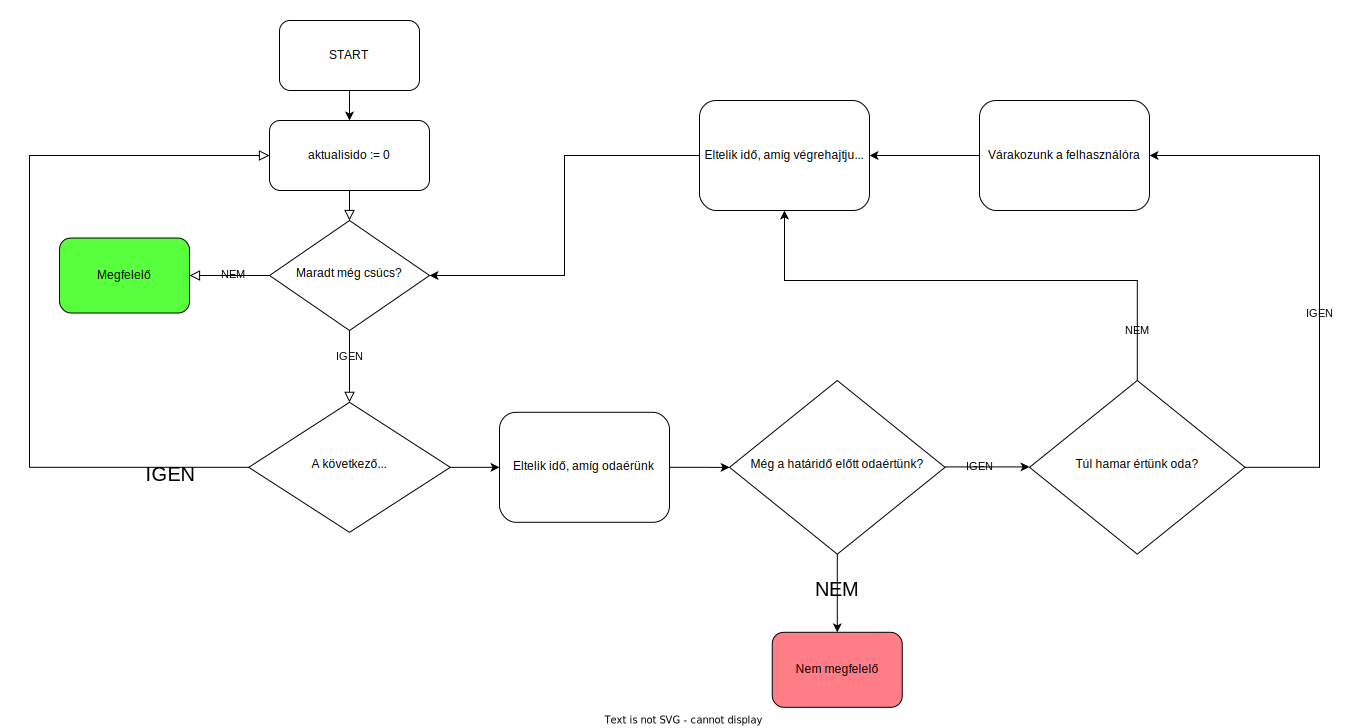
\includegraphics[width=150mm, keepaspectratio]{figures/timeWindow.drawio.png}
	\caption{A VRPTW során használt, időablak-feltételt kiértékelő függvény folyamatábrája}
	\label{fig:VRPTW_chart}
\end{figure}

\subsection{Kezdeti kudarcok}
Miután megvalósítottam és kipróbáltam a programot a kapott tesztadatokon (mérési eredmények az \ref{CVRPTW1section}. fejezetben), sajnálattal tapasztaltam, hogy 25 csúcsnál nagyobb gráfok esetében képtelen volt végeredményre jutni, illetve amiket sikerült is megoldani, azokat is rossz hatásfokkal tette.

\subsection{A probléma forrása} Az eredményekből az a következtetés vonható le, hogy a teljesen random közlekedő hangya nem alkalmas az algoritmus során olyan kezdeti megoldást találni, amit majd a következő hangya tovább tudna javítani. Az időablakok feltétele a kapacitással ellentétben közvetlenül a csúcsok sorrendjére szab meg korlátozást, vagyis gyakorlatilag lehetetlen pont a jó sorrendet eltalálni. 

\subsection{A megoldás felé vezető út}
A tesztadatokon látszik, hogy viszonylag rövid időintervallumokban lehet elérni az egyes felhasználókat. Ez azt jelenti, hogy ha egy jármű számára kiosztunk egy adott csúcshalmazt, akkor ezek permutációi közül csupán néhány lesz olyan, ami kielégíti az időablak-feltételt. Ha intuitívan közelítjük meg a helyzetet, akkor nagy valószínűséggel úgy járhatunk el a legjobban, hogyha a járműveknek sikertelenség esetén azt javasoljuk, hogy próbáljanak meg olyan ütemben haladni, ahogyan a csúcsok elérhetővé válnak.

\noindent
A teljesen random hangya elvét elhagyva \textit{\mbox{sortTrucksByReadyTime}} néven egy új függvényt írtam, amely minden járműhöz a ráosztott csúcshalmazt olyan sorrendbe állítja, ahogyan azok elérhetőek lesznek. Mivel csak rossz megoldásokat szűrök ki, a rendezéssel a megfelelő sorrendek halmazát vélhetően nem zavarom meg nagy mértékben.
